\documentclass{article}
\usepackage{graphicx} %package to manage images
\usepackage[utf8]{inputenc}
\usepackage[a4paper, total={6in, 8in}]{geometry}
\usepackage{xurl}
\title{Relatório 9 \\ Análise de transições}
\author{Pedro A. S. O. Neto}
\date{Maio, 2022}

\begin{document}

\maketitle

\section{Alternancia de fixações}

Calcula-se:

\begin{itemize}
  \item Número de transições (diretas e indiretas) entre objeto de interesse e rosto
  \item Número de transições diretas e indiretas entre rosto e objeto de interesse 
  \item Transições normalizadas (Transiçoes alvo-rosto - alvo-NãoRosto)/Total transições
\end{itemize}

%\begin{figure}[t]
%\caption{Abacaxi}
%\noindent\makebox[\textwidth]{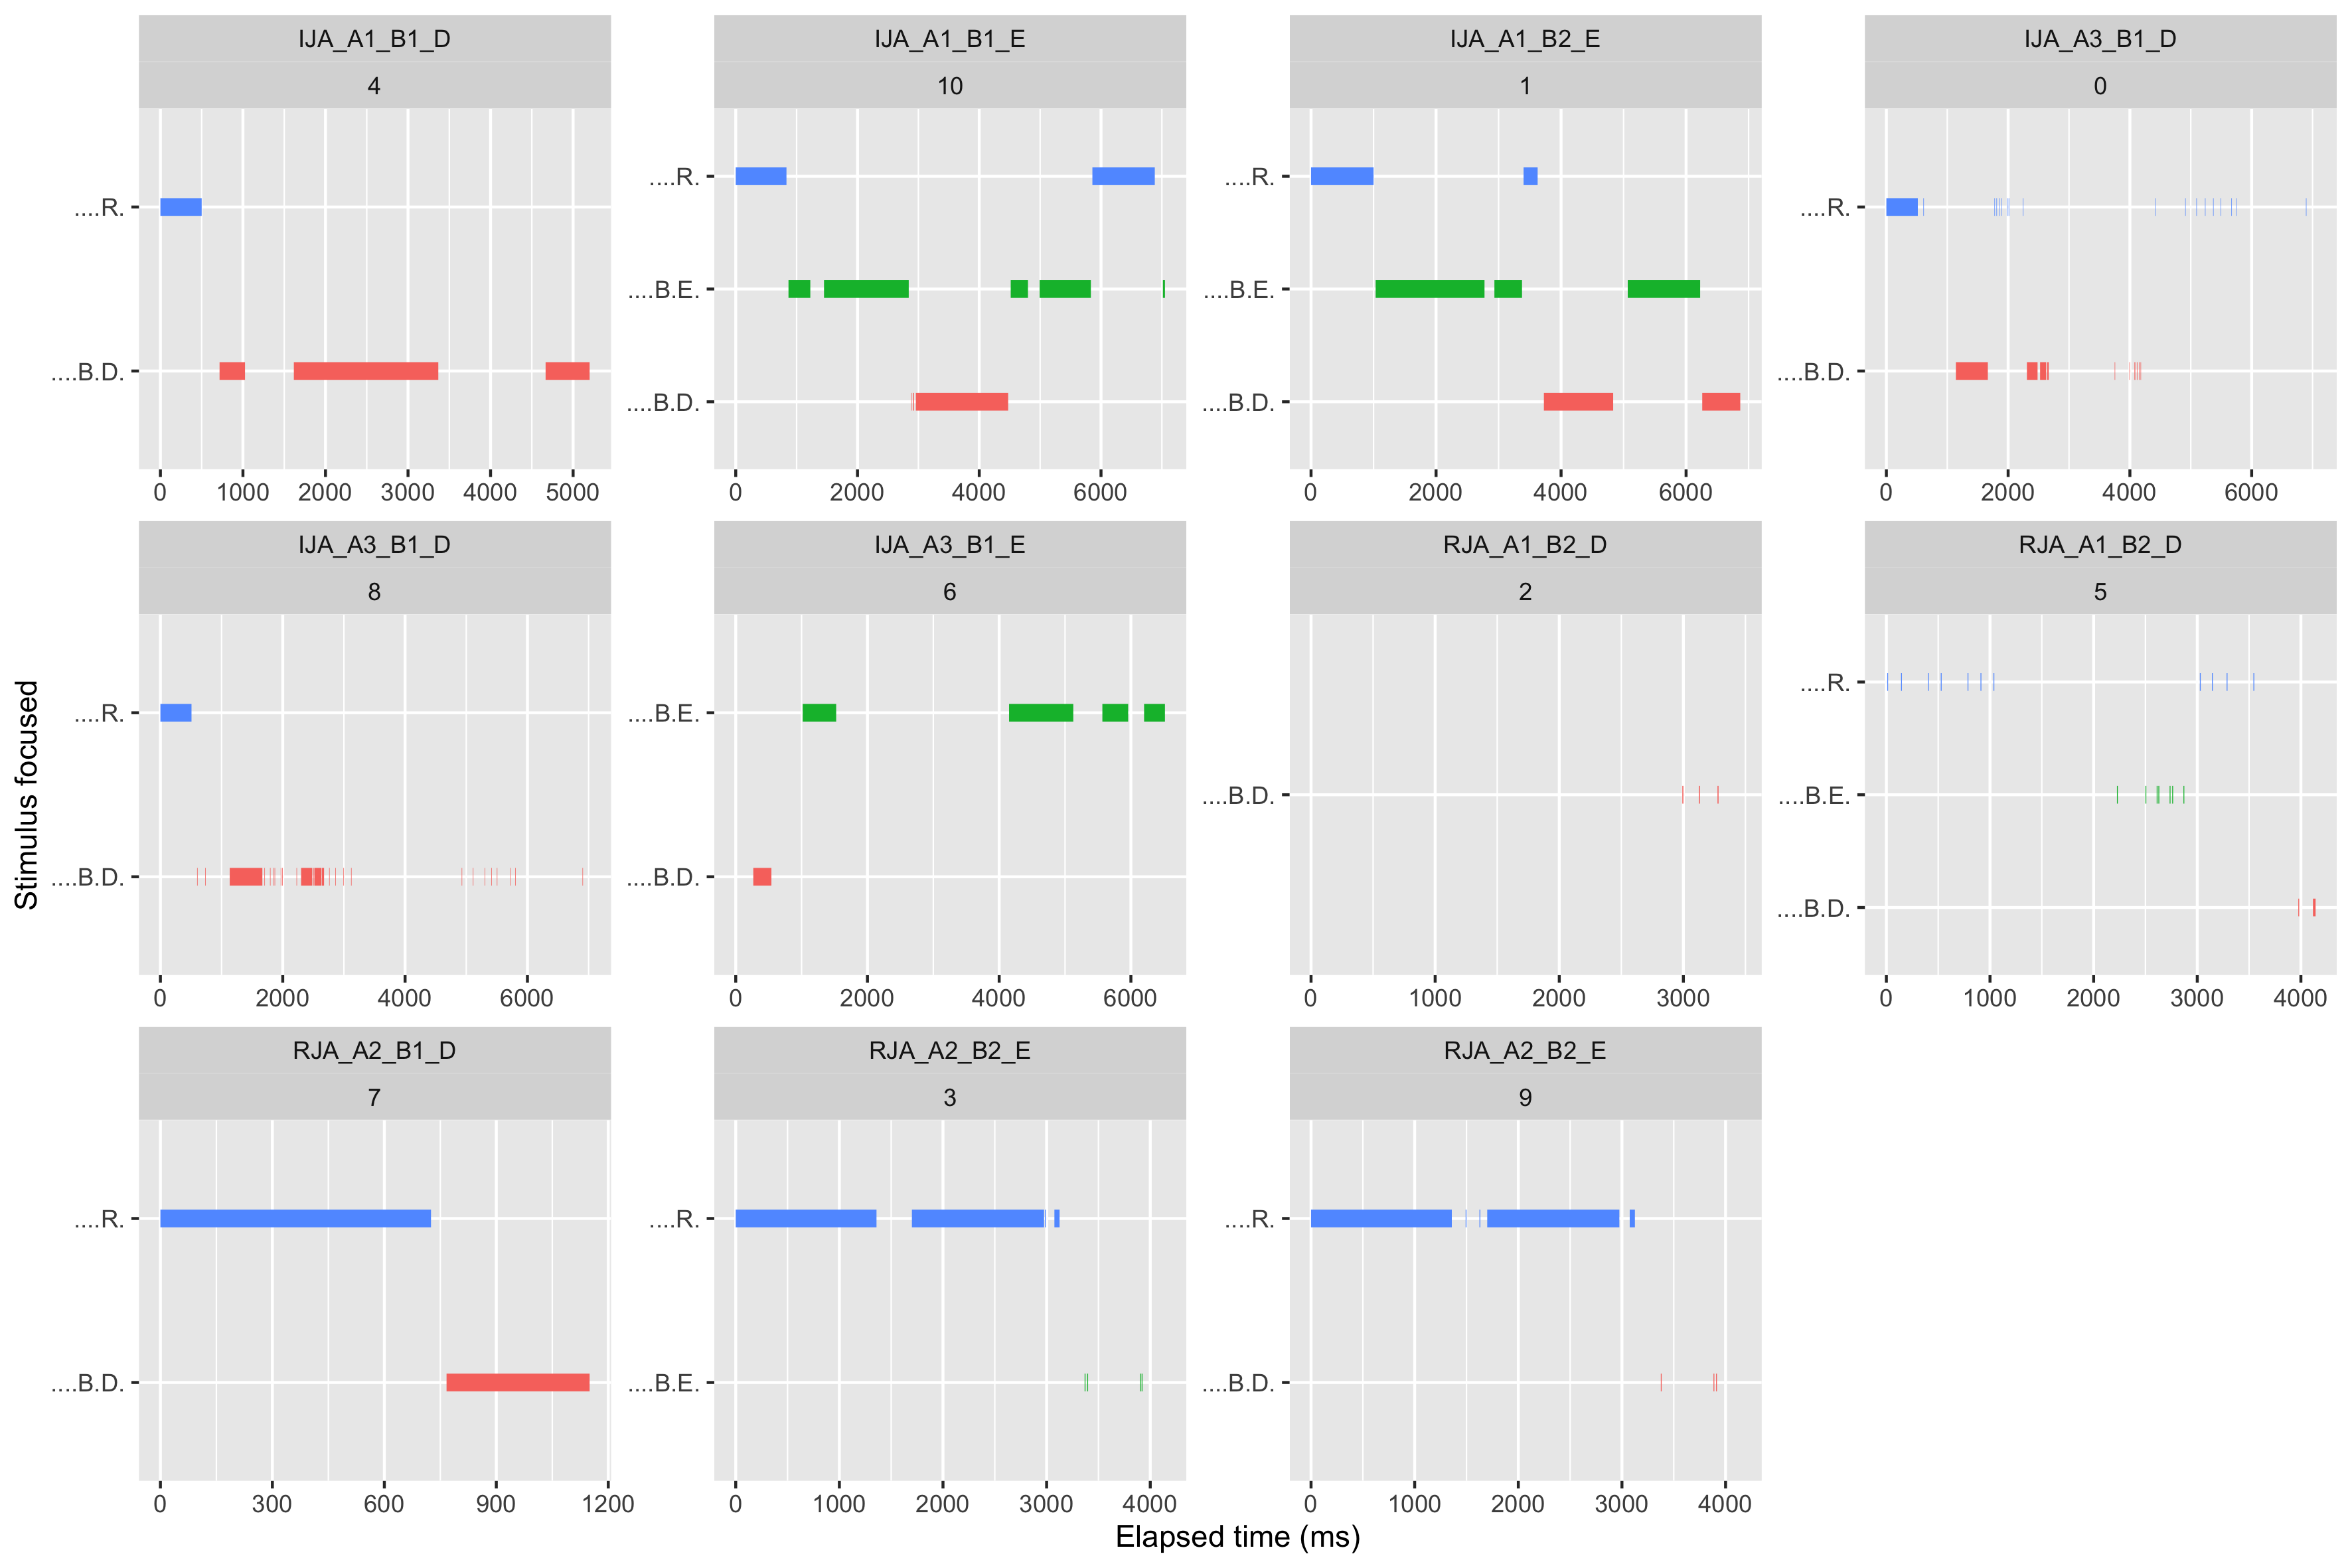
\includegraphics[width=\paperwidth]{"./graph_visu1.png"}}
%\centering
%\end{figure}


\end{document}
